\chapter*{Top heavy test distribution}

All but one of our tests are end-to-end tests, which is an example of a \emph{top heavy} test distribution. That might not seem such a big problem at the moment, but as the number of tests grows it will become an issue.

\QandAbox{What problems can you foresee if we don't address our test distribution?}{2}

\section*{Pushing tests down}

The Test Automation Pyramid is a metaphor created by Mike Cohn. If you're not familiar with it take a few minutes to read the appendix on page \pageref{testing-pyramid}

\QandAbox{What benefit do we get from running all our acceptance tests as end-to-end tests, at the top of the pyramid?}{2} 

\vbox{
Consider the schematic below again:
\begin{center}
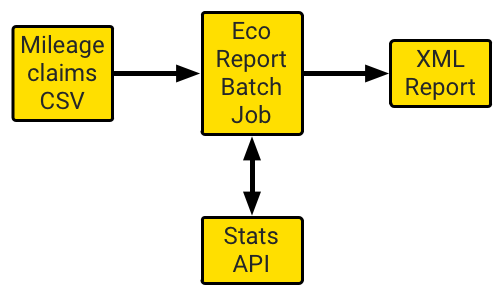
\includegraphics[height=8cm]{images/batch-job-overview-diagram}
\end{center}
}

Instead of reading the mileage claims from a CSV file, we could run tests by constructing a collection of mileage claims in memory and passing them to the \texttt{\ShoutyReportProcessor}. We could also compare the list of \texttt{\EcoStat} objects returned by \texttt{\ShoutyReportProcessor} in memory, without having to write an XML file. in fact, we could avoid interacting with the file system at all. This would make the tests faster, more reliable and more focused on a specific behaviour of the code.

We call this \emph{pushing tests down} the pyramid.

\QandAbox{Would you be concerned if we were left without any tests that read/write from/to the file system? Why?}{2} 

\vbox{
\section*{Move a test}

Now let's rewrite one of the end-to-end tests as a unit test. Move \texttt{single_sales_person()} from \texttt{\EndToEndTests} to \texttt{\UnitTests} and rewrite it to follow this pattern:

\begin{itemize}
    \item Create a \texttt{\FakeRevenueProvider} with required customers and revenues for the month
    \item Create a list of \texttt{\MileageClaim} objects
    \item Create a \texttt{\ShoutyReportProcessor}
    \item Call the \texttt{\ProcessMethod} method
    \item Assert that the list of \texttt{\EcoStat} objects returned is as expected
\end{itemize}
}

\QandAbox{Was writing the unit test easy? Is the test verbose or difficult to read?}{2}

\QandAbox{How could we improve the situation?}{2}